This section provides some information on 
implementation details of the adaptive optimization system.

Readers are encouraged to read the 
\xlink{2000 OOPSLA\begin{iftex}~\cite{jalapeno-adaptive-00}\end{iftex}}
{http://www.research.ibm.com/jalapeno/publication.html\#oopsla00\_aos}  
paper, which describes both the design and implmentation of the system
as of July 2000.


\subsection{System Architecture}
The RVM Adaptive Optimization System (AOS) contains three components, 
each of which encompasses one or more separate threads of control. 
These subsystems are 
the {\em runtime measurements subsystem\/}, 
the {\em controller\/},  
and the {\em recompilation subsystem\/}.  
Figure~\ref{fig:arch-AOSOverview} depicts the internal structure of
the RVM adaptive optimization system and the interactions between its
components. 
In addition to the components, the {\em AOS database} provides a 
repository that records component decisions and allows components 
to query these decisions.
The next four sections discuss this figure in more detail.

\begin{figure}
\begin{center}
\begin{gif}{arch-AOSOverview}
\vbox{
\hbox{
\psfig{file=arch-AOSOverview.ps,width=\textwidth}
%height=5in}
}
}\hfil
\end{gif}
\end{center}
\caption{Architecture of the Adaptive Optimization System}
\label{fig:arch-AOSOverview}
\end{figure}

The controller thread (in vm/adaptive/controller/VM\_ControllerThread)
is created during RVM boot time.  It subsequently creates threads
corresponding to the other subsystems: organizer threads to perform
sample-based runtime measurements and a single compilation thread to
perform recompilation. After these threads are created, the controller
sleeps until the runtime measurements subsystem inserts an event in
the organizer event queue.

The adaptive optimization system (without adaptive inlining) creates
an organizer thread, a {\em method sampler organizer\/}.  This
organizer processes method samples and inserts events in the organizer
event queue to allow the controller to consider the methods for
recompilation.

When adaptive inlining is enabled (it is by default), a decay
organizer is created.  This decay organizer decays counters associated
with call graph edges using for adaptive inlining.  The decay
organizer does not communicate directly with the controller.


\subsection{Runtime Measurements Subsystem}\label{sec:arch:rms}
The runtime measurements subsystem gathers information
about the executing methods, summarizes the information, and then
either passes the summary along to the controller via the organizer
event queue or records the information in the AOS database.

Figure~\ref{fig:arch-AOSOverview} shows the structure of the runtime
measurements subsystem.  
Several systems, including 
instrumentation in the executing
code, 
hardware performance monitors, and VM instrumentation, 
produce
raw profiling data as the program runs.
Usually, these systems perform only extremely limited processing of the
raw data as it is produced.
Instead, separate threads called {\em organizers} periodically 
process and analyze the raw data.
The design separates the generation of raw profiling data from the 
data analysis for two reasons.  First, this design allows
multiple organizers to process the same raw data, possibly in
different ways. Second, this separation allows low-level profiling
code to execute under strict resource constraints.  Recall that
we monitor not just application code, but also system services of the 
VM. So, for example, 
low-level code that monitors the VM memory allocator must not allocate 
any objects (it must use
pre-allocated data structures and buffers) and should complete its
task in a short time period.

The controller directs the data monitoring and creates
organizer threads to process the raw data at specific time
intervals. When awoken, each organizer analyzes raw data, and
packages the data into a suitable form for consumption by the
controller.  Additionally, an organizer may add
information to the organizer event queue for the controller to
process, or may record information in the AOS database for later
queries by other AOS components.

The sampling implementation takes advantage of existing mechanisms in
RVM.  Before switching threads, a counter associated with the current
method is incremented.  The system attributes a sample taken on a back
edge to the current method.  A sample taken in a method prologue is
credited to both the calling and current method, capturing the fact
that control is in transition between both methods. 

This sampling technique provides a basic mechanism to estimate the
time spent in execution of each method.  In the adaptive optimization
system, two organizer threads periodically process the raw data.

The first organizer thread (the {\em method sampler organizer}), created
during system startup, installs a sampling object (the {\em method
listener}) to record raw data regarding the execution profile.
During a thread switch, the
VM invokes the {\tt update} method of this listener, which records the
currently active method in a raw data buffer. 
This activity costs only a few
additional cycles during each thread switch, and the performance
impact does not stand out from noise from one run to the next.
After collecting the number of samples specified by its current sample
size, the method listener wakes the hot methods organizer thread. 

When awoken, the hot methods organizer scans the method counter raw data to
identify methods where the application spends most of its time. 
For each hot method it
discovers, the hot methods organizer enqueues an event
in the organizer event queue.

\subsection{Controller}\label{sec:arch:control}
The controller orchestrates and conducts the other components of 
the adaptive optimization system.
It coordinates the activities of the runtime measurements subsystem
and the recompilation subsystem.
The controller initiates all runtime measurement subsystem profiling 
activity by determining what profiling should occur, under what conditions,
and for how long.
It receives information from the runtime measurement subsystem and AOS
database, and uses this information to make compilation decisions.
It passes these compilation decisions to the recompilation subsystem,
directing the actions of the various compilers.

Based on information from the runtime measurements subsystem and the 
AOS database, the controller can perform the following actions: 
1) it can instruct the runtime measurements subsystem to
continue or change its profiling strategy, which could include using
the recompilation subsystem to insert intrusive profiling; 2) it can
recompile one or more methods using profiling data to improve their
performance.  The controller makes these decisions based on an
analytic model representing the costs and benefits of performing these
tasks.

The controller communicates with the other two components using
priority queues; it extracts measurement events from a queue that is
filled by the runtime measurements subsystem and inserts recompilation
decisions into a queue that compilation threads process.  When
these queues are empty, the dequeuing thread(s) sleep.  The various
system components also communicate 
indirectly by reading and writing information in the AOS database.

\subsection{Recompilation Subsystem}\label{sec:arch:comp}
The recompilation subsystem consists of compilation threads that
invoke compilers.
The compilation threads extract and execute compilation plans
that are inserted into the compilation queue by the controller. 
Recompilation occurs in separate threads from the application, and thus, 
can occur in parallel. 
This differs from the initial (lazy) compilation of a method, 
which occurs the first time a method is invoked:
during lazy compilation, compilation occurs in the application 
thread that attempted to invoke the uncompiled method.

Each compilation plan consists of three components: an {\em optimization
plan\/}, {\em profiling data\/}, and an {\em instrumentation plan\/}.
The optimization plan specifies which optimizations the compiler
should apply during recompilation.  
The profiling data, initially gathered by the runtime measurements subsystem, 
directs the optimizing compiler's feedback-directed optimizations.  
Instrumentation plans dictate which, if any, intrusive instrumentation the compiler 
should insert into the generated code. 

The compilation threads takes the output of the compiler --- an
object that represents the executable code and associated runtime
information (exception table information and garbage collection maps) ---
and installs it in the RVM, so that all future calls to this method
will use the new version.  In our current implementation, any previous
activations of the method will continue to use the old compiled
code for the method until that method's activation completes.  Nothing
in our design precludes using stack frame rewriting to enable previous
activations of the method to use the new compiled version, but this
functionality has not yet been implemented.  We expect that RVM will
eventually rewrite baseline stack frames to optimized stack frames. 
It is as yet unclear if there is sufficient motivation to support
the more difficult transition between two optimized stack frames. 


\subsection{AOS Database}\label{sec:arch:db}
The AOS database provides a repository where the adaptive optimization 
system 
records decisions, events, and static analysis results. The various adaptive 
system components query these artifacts as needed. 

For example, the controller uses the AOS database to record
compilation plans and to track the status and history of methods
selected for recompilation.  The controller and organizer threads
query this information as needed to guide recompilation decisions.


\subsection{Adaptive Inlining}
This section describes an extension to the adaptive optimization
system to support online feedback-directed inlining.
At a high level, the system takes a statistical
sample of the method calls in the running application and maintains
an approximation to the dynamic call graph based on this data.
Using this approximate dynamic call graph, the system identifies
``hot'' edges to inline, and passes the information to the optimizing
compiler.  The system may choose to recompile already optimized
methods to inline hot call edges. 

When a thread switch occurs in a method prologue, the system calls the
{\tt update} method of an {\em edge listener} (as well as the method
listener as discussed in Section~\ref{sec:arch:rms}).  This edge
listener walks the thread's stack to determine the call site that
originated the call.  The edge listener creates a tuple identifying
the calling edge (specified by the caller, call site, and callee) and
inserts this tuple into a buffer.

When the buffer becomes full, the edge listener is temporarily
deactivated (its update method will not be called again at a prologue
thread switch) and it
notifies the 
{\em dynamic call graph (DCG) organizer} to wake up and process the
buffer. The DCG organizer maintains a dynamic call graph, where each 
edge corresponds to a tuple value in the buffer. After updating the
weights in the dynamic call graph, the DCG organizer clears the
buffer, and reactivates the edge listener.
The decay organizer, a separate thread, periodically decays the edge
weights in the dynamic call graph.

Periodically, the DCG organizer invokes the {\em adaptive inlining
organizer} to recompute adaptive inlining decisions.  The adaptive
inlining organizer performs two functions.  First,
it identifies edges in
the dynamic call graph whose percentage of samples exceed an edge
hotness threshold. 
These edges are added to an {\em inlining rules} data structure,
which is consulted by the controller when it formulates
compilation plans.  Any edge in this data structure
will be inlined if the calling method is subsequently recompiled,
subject to generous size constraints.
The system sets the initial edge hotness threshold 
fairly high, but periodically reduces it until reaching a
fixed minimal value.  Effectively, this forces 
inlining to be more conservative 
during program startup, but allows it to become progressively more
aggressive as profiling data accumulates. 

The second function of the adaptive inlining organizer is to identify
methods that are candidates for further recompilation to enable
inlining of hot call edges. To be identified as a recompilation
candidate by the inlining organizer, a method must satisfy two
criteria.  First, the method must be hot, as defined by the hotness
threshold used by the hot method organizer.  Second, recompiling
the method must force a new inlining action, as dictated by the 
inlining rules data structure.

When the adaptive inlining organizer identifies a method for recompilation,
it enqueues an event representing the method for consideration by the
controller.  

